\documentclass[../main.tex]{subfiles}

\makeatletter
\@ifundefined{fromRoot}{%
  \newcommand{\fromRoot}[1]{../#1}
  
  % \usepackage{xr}
  % \externaldocument{../main}
}{}

\def\input@path{{\subfix{../}}}
%or: \def\input@path{{/path/to/folder/}{/path/to/other/folder/}}
\makeatother

\graphicspath{
  {\subfix{../}}
  {\subfix{./figures}}
  {\subfix{../figures}}
  {\subfix{./figures/logos-thesis/}}
  {\subfix{../figures/logos-thesis/}}
  {\subfix{./figures/rtexps-pics/}}
  {\subfix{../figures/rtexps-pics/}}
}


\hypersetup{
    pdfauthor   = {Camille MONIÈRE},
    pdftitle    = {Th\`{e}se (Présentation: QCSP, un résumé)},
    pdfsubject  = {Th\`{e}se (Présentation: QCSP, un résumé)},
%    pdfkeywords = {mots-cl\'{e}s},
}

\begin{document}


\section[\acrshort{qcsp}]{Le projet \acrfull{qcsp}}

\begin{frame}{\secname}{\href{https://qcsp.univ-ubs.fr/}{https://qcsp.univ-ubs.fr/}}

  \begin{columns}
    \begin{column}{.4\linewidth} \centering
      \begin{columns}
        \begin{column}{.4\linewidth}
          
\includegraphics[width=\textwidth]{QCSP_Logo.pdf}
        \end{column}
        \begin{column}{.2\linewidth}
          
\includegraphics[width=\linewidth]{anr_approved.jpg}
        \end{column}
      \end{columns}
      \small \vspace{5pt} Projet ANR \texttt{ANR-19-CE25-0013-01}
    \end{column}
    \begin{column}{.5\linewidth}
      \emph{``L'objectif du projet QCSP est de contribuer à l'évolution des réseaux IoT en établissant,
        en mettant en œuvre et testant un nouveau type de modulation codée.''}
    \end{column}
  \end{columns}

  \vspace{2 em}

  \begin{center}
    Partenaires :\\
    
\includegraphics[width=0.6\linewidth]{figures/logos-thesis/partners-logos.png}
  \end{center}
  \note{
    \begin{enumerate}
      \item QCSP, sa vie, son oeuvre (C'est quoi, but, idée)
      \item Les partenaires : 
      \begin{itemize}
        \item IMT, CEA, Autres labsticc : Code correcteur d'erreur (Turbo/ldpc/polar NB)
        \item Orange : IA et valolo
        \item LIU, LabSTICC : l'algo
        \item Moi : Faisabilité temps réel 
      \end{itemize}
    \end{enumerate}
  }
\end{frame}


\subsection[\acrshort{ccsk}]{\acrfull{ccsk}}

\begin{frame}{\acrfull{ccsk}}
  {}
  % \begin{overlayarea}{\linewidth}{.02 \textheight}
  % \end{overlayarea}
  \begin{overlayarea}{\linewidth}{.15 \textheight} \centering
    symboles de $p$ bits $\Longrightarrow$ rotation circulaire d'une \emph{séquence de pseudo-bruit binaire} \pn{0} \cite{dillardCyclicCodeShift2003}.\\
    \pn{0} est composée de $2^p = q$ \emph{chips}, telle que $\mpn{0} = [P_0(0), ..., P_0(q - 1)]$
  \end{overlayarea}

  \begin{columns}
    \begin{column}{.3\linewidth}
      \begin{overlayarea}{\linewidth}{.37 \textheight}
        \centering

        \begin{tabular}{@{}r r l@{}}
          \toprule
          \multicolumn{3}{c}{\textbf{Paramètres}}         \\ \midrule
          $p$    & $=$ & $2$ bits par symbole             \\
          $q$    & $=$ & $4$ symboles possibles           \\
          \pn{0} & $=$ & \Ob{}\Xb{}\Xb{}\Xb{} ($4$ chips) \\
          \bottomrule
        \end{tabular} \vspace*{-2pt}

        \Ob{} $= 1$, \Xb{} $= 0$
      \end{overlayarea}
    \end{column}
    \begin{column}{.3\linewidth}
      \begin{overlayarea}{\linewidth}{.37 \textheight}
        \begin{tabular}{@{}r c l@{}}
          \toprule
          \textbf{Symbole} & \textbf{Notation} & \textbf{Rotation}    \\ \midrule
          $0$              & \pn{0}            & \Ob{}\Xb{}\Xb{}\Xb{} \\
          $1$              & \pn{1}            & \Xb{}\Ob{}\Xb{}\Xb{} \\
          $2$              & \pn{2}            & \Xb{}\Xb{}\Ob{}\Xb{} \\
          $3$              & \pn{3}            & \Xb{}\Xb{}\Xb{}\Ob{} \\
          \bottomrule
        \end{tabular}
      \end{overlayarea}
    \end{column}
  \end{columns}

  \vspace{1 em}

  \begin{columns}
    \begin{column}{.35\linewidth}
      \begin{overlayarea}{\linewidth}{.19 \textheight}
        \centering
        Mot de code $\vect{C}$ de $3$ symboles\\
        $\{ 0, \; 3, \; 1\}$
      \end{overlayarea}
    \end{column}
    \begin{column}{.05\linewidth}
      \centering
      $\Rightarrow$
    \end{column}
    \begin{column}{.6\linewidth}
      \begin{overlayarea}{\linewidth}{.19 \textheight}
        \centering
        % \begin{noindent}
        \begin{tabular}{@{}r c@{}}
          \multicolumn{2}{c}{Trame \acrshort{ccsk} $\vect{F}_{CCSK}$}          \\
          $\{ \mpn{0} \;|\; \mpn{3} \;|\; \mpn{1} \}$ = 
            & {\large \Ob{}\Xb{}\Xb{}\Xb{}~~\Xb{}\Xb{}\Xb{}\Ob{}~~\Xb{}\Ob{}\Xb{}\Xb{}} \\
            & \includegraphics[width=.387\linewidth, height=.05\textheight]{figures/tikzpicture/pn_chrono.pdf}
        \end{tabular}
        % \end{noindent}
      \end{overlayarea}
    \end{column}
  \end{columns}
  \begin{columns}
    \begin{column}{.6678\linewidth}
      Après le CCSK, on applique une BPSK ($1 \rightarrow +1$, $0 \rightarrow -1$) :
    \end{column}
    \begin{column}{.2322\linewidth} \centering
      \includegraphics[width=\linewidth, height=.1\textheight]{figures/tikzpicture/pn_chrono_bpsk.pdf}
    \end{column}
    \begin{column}{.055\linewidth}
    \end{column}
  \end{columns}
  \blfootnotetext{\textcite{dillardCyclicCodeShift2003}}
  % \footnotetext{Corps de Galois d'ordre $p$}
  \note{
    \begin{enumerate}
      \item CCSK c'est important
      \item comme dis avant ... envoyer des bits n'est pas fiables -> on module
      \item on dis que P0 c'est des 'chips' pour bien faire la distinction avec les bits d'informations
      \item on prend groupe de bits -> symbole -> rotation de P0
      \item déroule BG
    \end{enumerate}
  }
\end{frame}

\begin{frame}{\acrshort{ccsk} : Démodulation}
  {\scriptsize Note : Post BPSK, donc cette fois, \Ob{} $= +1$, \Xb{} $= -1$.}

  Corrélation circulaire $\vect{L}$: $\quad\forall k \in \llbracket 0, q - 1 \rrbracket, \quad L(k) = \sum_{i = 0}^{q - 1} y(i) \times P_0(k + i \mod{q})$. \vspace{-2pt}
  \begin{center}
    On note $\vect{y} = \mgb{} \mgb{} \mgb{} \mgb{}$, avec ``$\mgb{}$'' une valeur quelconque.
  \end{center} \vspace{-5pt}
  \begin{columns}
    \begin{column}{.25\linewidth}
      \centering
      \ra{.5}
      \begin{tabular}{@{}r l@{}}
        $L(0) =$ &
        \begin{tabular}{@{}c l@{}}
          $\mgb{} \pta{} \mgb{} \pta{} \mgb{} \pta{} \mgb{}$ \\
          $\times + \times + \times + \times$                \\
          $\mOb{} \pta{} \mXb{} \pta{} \mXb{} \pta{} \mXb{}$
        \end{tabular}
      \end{tabular}
      \ra{1}
    \end{column}
    \begin{column}{.25\linewidth}
      \centering
      \ra{.5}
      \begin{tabular}{@{}r l@{}}
        $L(1) =$ &
        \begin{tabular}{@{}c@{}}
          $\mgb{} \pta{} \mgb{} \pta{} \mgb{} \pta{} \mgb{}$ \\
          $\times + \times + \times + \times$                \\
          $\mXb{} \pta{} \mOb{} \pta{} \mXb{} \pta{} \mXb{}$
        \end{tabular}
      \end{tabular}
      \ra{1}
    \end{column}
    \begin{column}{.25\linewidth}
      \centering
      \ra{.5}
      \begin{tabular}{@{}r l@{}}
        $L(2) =$ &
        \begin{tabular}{@{}c@{}}
          $\mgb{} \pta{} \mgb{} \pta{} \mgb{} \pta{} \mgb{}$ \\
          $\times + \times + \times + \times$                \\
          $\mXb{} \pta{} \mXb{} \pta{} \mOb{} \pta{} \mXb{}$
        \end{tabular}
      \end{tabular}
      \ra{1}
    \end{column}
    \begin{column}{.25\linewidth} \centering
      \ra{.5}
      \begin{tabular}{@{}r l@{}}
        $L(3) =$ &
        \begin{tabular}{@{}c@{}}
          $\mgb{} \pta{} \mgb{} \pta{} \mgb{} \pta{} \mgb{}$ \\
          $\times + \times + \times + \times$                \\
          $\mXb{} \pta{} \mXb{} \pta{} \mXb{} \pta{} \mOb{}$
        \end{tabular}
      \end{tabular}
      \ra{1}
    \end{column}
  \end{columns}

  \vspace{7pt}

  \hrule{}

  \vspace{7pt}

  \begin{columns}
    \begin{column}{.25\linewidth}
      \captionof{figure}{$\vect{y} = \mpn{0}$ \\ Autocorrélation circulaire de \pn{\textcolor{Red}{\bm{0}}}}
      \includegraphics[width=\linewidth]{pgfplots/pn_demod_0.pdf}
    \end{column}
    \begin{column}{.25\linewidth}
      \captionof{figure}{$\vect{y} = \mpn{1}$ \\ Corrélation circulaire de \pn{0} et \pn{\textcolor{Red}{\bm{1}}}}
      \includegraphics[width=\linewidth]{pgfplots/pn_demod_1.pdf}
    \end{column}
    \begin{column}{.25\linewidth}
      \captionof{figure}{$\vect{y} = \mpn{2}$ \\ Corrélation circulaire de \pn{0} et \pn{\textcolor{Red}{\bm{2}}}}
      \includegraphics[width=\linewidth]{pgfplots/pn_demod_2.pdf}
    \end{column}
    \begin{column}{.25\linewidth}
      \captionof{figure}{$\vect{y} = \mpn{3}$ \\ Corrélation circulaire de \pn{0} et \pn{\textcolor{Red}{\bm{3}}}}
      \includegraphics[width=\linewidth]{pgfplots/pn_demod_3.pdf}
    \end{column}
  \end{columns}
  \note{
    \begin{enumerate}
      \item D'abord lis (comme à l'entrainement)
      \item Oublie pas, si $y \ncong \mpn{0}$, y.a.r. 
    \end{enumerate}
  }
\end{frame}

\subsection{Modèle}

\begin{frame}{\secname : \subsecname}
  \begin{overlayarea}{\linewidth}{0.25\textheight}
    \resizebox{\linewidth}{!}{
      \begin{tikzpicture} [-latex,
    >=latex,
    auto,
    thick,
    main node/.style={rectangle, fill = white!35, draw,
        align=center}
  ]

  \node [main node,
    visible on=<1>,
    fill = red!20!white,
    align=center,
    minimum height = 1.5cm
  ] (nbenc_HL) at (0, 0) {Encodeur\\NB-LDPC};

  \node [main node,
    visible on=<2->,
    align=center,
    minimum height = 1.5cm
  ] (nbenc) at (0, 0) {Encodeur\\NB-LDPC};

  \node [main node,
    visible on=<2>,
    fill = red!20!white,
    minimum height = 1.5cm,
    right = 1cm of nbenc
  ] (ccskm) {Modulation\\CCSK};

  \node [main node,
    visible on=<3->,
    minimum height = 1.5cm,
    right = 1cm of nbenc
  ] (ccskm) {Modulation\\CCSK};

  \node [main node,
    visible on=<3>,
    fill = red!20!white,
    minimum height = 1.5cm,
    minimum width = 2cm,
    right = 1cm of ccskm
  ] (bpskm) {BPSK};% $+$\\Surmodulation};

  \node [main node,
    visible on=<4->,
    minimum height = 1.5cm,
    minimum width = 2cm,
    right = 1cm of ccskm
  ] (bpskm) {BPSK};% $+$\\Surmodulation};

  \node [main node,
    visible on=<4>,
    fill = red!20!white,
    minimum height = .75cm,
    minimum width = .5cm,
    right = 1 cm of bpskm
  ] (dac) {Filtre $+$ CNA};

  \node [diamond,
    visible on=<4>,
    fill = red!20!white,
    draw,
    align=center,
    %minimum height = 1.5cm,
    %minimum width = 2cm,
    right = .5 cm of dac
  ] (chan) {Canal};

  \node [main node,
    visible on=<4>,
    fill = red!20!white,
    minimum height = .75cm,
    minimum width = .5cm,
    right = .5cm of chan
  ] (adc) {CAN $+$ Filtre};


  \node [diamond,
    aspect = 2,
    draw,
    visible on=<5->,
    minimum height = .75cm,
    minimum width = .5cm,
    fill = white,
    align = center,
  ] (bichan) at (chan) {Canal gaussien\\complexe asynchrone};


  \node [main node,
    visible on=<6>,
    fill = red!20!white,
    minimum height = 1.5cm,
    %minimum width = 3cm,
    right = 1 cm of adc
  ] (ccskd)  {Détection};

  \node [main node,
    visible on=<7->,
    minimum height = 1.5cm,
    %minimum width = 3cm,
    right = 1 cm of adc
  ] (ccskd)  {Détection};

  \node [main node,
    visible on=<7>,
    fill = red!20!white,
    minimum height = 1.5cm,
    %minimum width = 3cm,
    right = 1 cm of ccskd
  ] (ccsks) {Synchronisation};

  \node [main node,
    visible on=<8->,
    minimum height = 1.5cm,
    %minimum width = 3cm,
    right = 1 cm of ccskd
  ] (ccsks) {Synchronisation};

  \node [main node,
    visible on=<8->,
    fill = red!20!white,
    minimum height = 1.5cm,
    right = 1cm of ccsks
  ] (nbdec) {Decodeur\\NB-LDPC};

  %%%%%%%%%%%%%%%%%%%%%%%%%%%%%%

  \draw  [visible on=<1->] ($(-1, 0) + (nbenc.west)$) -> (nbenc.west)
  node [visible on=<1->, pos=0, align=center, below = 1cm] (M) {Message\\$\vect{M}$\\($K \times p$ bits)};
  \draw [visible on=<1->] (nbenc.east) -> (ccskm.west)
  node [visible on=<1->, midway, align=center, below = 1cm] (M) {Mot de code\\$\vect{C}$\\($N \times p$ bits)};
  \draw [visible on=<2->] (ccskm.east) -> (bpskm.west)
  node [visible on=<2->, midway, align=center, below = 1cm] (M) {Trame CCSK\\$\vect{F}_{\mathrm{CCSK}}$\\($N \times q$ bits)};
  \draw [visible on=<3-4>] (bpskm.east) -- (dac.west)
  node [visible on=<3-4>, midway, align=center, below = 1cm] (TQ) {Trame QCSP\\$\vect{F}$\\($N \times q$ chips)};
  \draw [visible on=<4>] (dac.east) -- (chan.west);
  \draw [visible on=<4>] (chan.east) -- (adc.west);
  \draw [visible on=<4>] (adc.east) -- (ccskd.west)
  node [visible on=<4>, midway, align=center, below = 1cm] (M) {Échantillons\\$y(n)$\\($1 \times \mathcal{O}$ échantillons)};
  \draw [visible on=<5->] (bpskm.east) -- (bichan.west);
  \node [visible on=<5->, align=center, ] at (TQ) {Trame QCSP\\$\vect{F}$\\($N \times q$ chips)};
  \draw [visible on=<5->] (bichan.east) -- (ccskd.west);
  \node [visible on=<5->, align=center,] at (M) {Échantillon\\$y(n)$\\($1$ chip)};
  \draw [visible on=<6->] (ccskd.east) -> (ccsks.west)
  node [visible on=<6->, midway, align=center, below = 1cm] (M) {\phantom{É}Trame détectée\phantom{É}\\$\vect{F}_D$\\($2  N \times q$ chips)};

  \draw [visible on=<7->] (ccsks.east) -> (nbdec.west)
  node [visible on=<7->, midway, align=center, below = 1cm] (M) {\phantom{É}Trame synchronisée\phantom{É} \\ $\vect{F}_s$\\ ($N \times q$ chips)};

  \draw [visible on=<8->] (nbdec.east) -> ($(1, 0) + (nbdec.east)$)
  node [visible on=<8->, pos=1, align=center, below = 1cm] (M) {\phantom{É}Message décodé\phantom{É}\\$\vect{M}'$\\($K \times p$ bits)};

  \draw [visible on=<2->, latex-latex] ($(0, .2) + (nbenc.north west)$) -- ($(0, .2) + (ccskm.north east)$)
  node [midway, align=center, above = .2cm] (Mp) {Taux réel de codage : $R_{eff} = \frac{K \times p}{N \times q}$};

\end{tikzpicture}

    }
  \end{overlayarea}

  \vspace{1 em}
  \begin{columns}
    \begin{column}{.3\linewidth}
      \begin{overlayarea}{\linewidth}{0.6\textheight}
        \only<1->{\hfill Message $\vect{M}$\\} \vspace{.25em}
        \only<1->{\hfill Mot de code $\vect{C}$\\} \vspace{.25em}
        \only<2->{\hfill Trame CCSK $\vect{F}_{\mathrm{CCSK}}$\\} \vspace{.25em}
        \only<3->{\hfill Trame QCSP $\vect{F}$\\} \vspace{.25em}
        \only<4->{\hfill Flux d'échantillons $y(n)$\\} \vspace{.25em}
        \only<6->{\hfill Trame détecté $\vect{F}_{D}$\\} \vspace{.25em}
        \only<7->{\hfill Trame synchronisation $\vect{F}_{S}$\\} \vspace{.25em}
        \only<8->{\hfill Mode de code reçu $\vect{C}'$} \vspace{.25em}
        \only<9->{\hfill Message décodé $\vect{M}'$}
      \end{overlayarea}
    \end{column}
    \begin{column}{.7\linewidth}
      \begin{overlayarea}{\linewidth}{0.6\textheight} \centering
        \only<1->{$\{1, \: 2, \: 1\}$\\} \vspace{.25em}
        \only<1->{$\{1, \: 2, \: 1, \: 3, \: 2, \: 3\}$\\} \vspace{.25em}
        \only<2>{\includegraphics[width=\linewidth, height=.73em, keepaspectratio = true]{figures/tikzpicture/trame_ccsk.pdf}\\}% \vspace{.25em}
        \only<3->{\vspace{.5em} \includegraphics[width=\linewidth, height=2.19em, keepaspectratio = true]{figures/tikzpicture/trame_qcsp.pdf}\\} \vspace{.25em}
        \only<4->{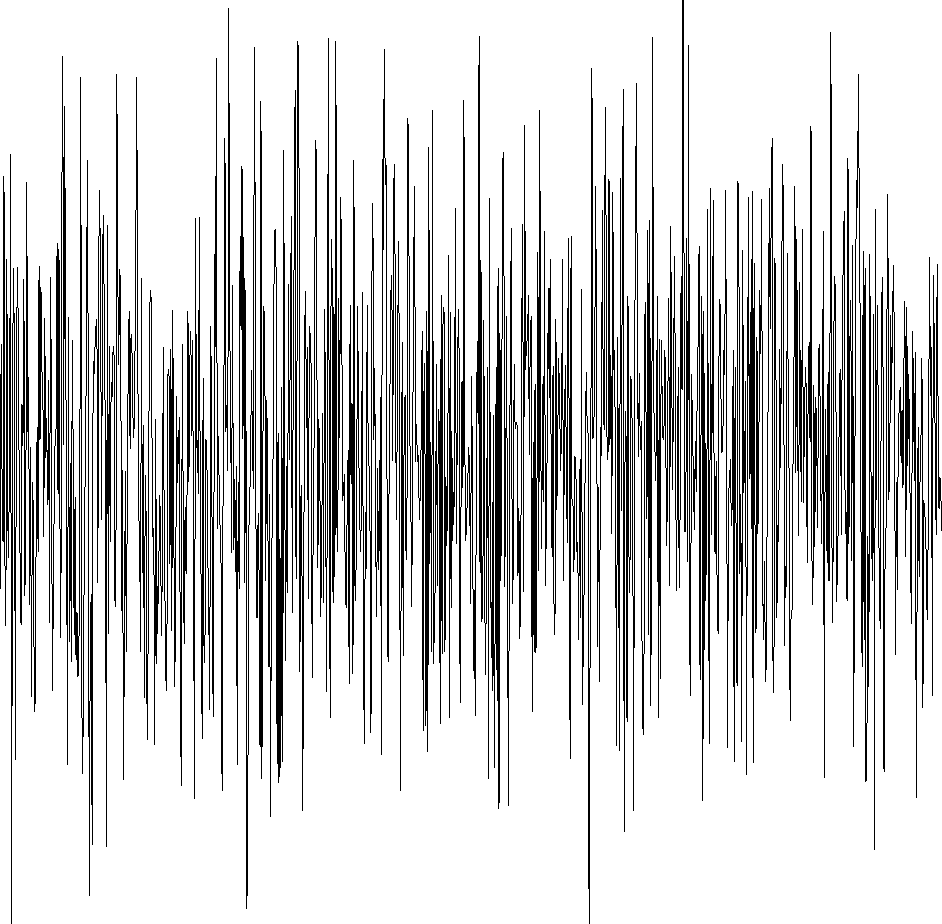
\includegraphics[width=\linewidth, height=.73em, keepaspectratio = false]{figures/rtexps-pics/noise.png}\\} \vspace{.25em}
        \only<6->{\includegraphics[width=\linewidth, height=1.05em, keepaspectratio = true]{figures/tikzpicture/trame_detectee.pdf}\\} \vspace{.25em}
        \only<7->{\includegraphics[width=\linewidth, height=1.05em, keepaspectratio = true]{figures/tikzpicture/trame_synchro.pdf}\\} \vspace{.25em}
        \only<8->{$\{1, \: \textcolor{Red}{0}, \: 2, \: \textcolor{Red}{0}, \: 2, \: 3\}$\\}
        \vspace{.25em}
        \only<9->{$\{1, \: 2, \: 1\}$}
      \end{overlayarea}
    \end{column}
  \end{columns}
\end{frame}

\subsection{Détection}

\begin{frame}{\subsecname~basée sur la CCSK}
  \begin{columns}
    \begin{column}{.6\linewidth}
      \begin{overlayarea}{\linewidth}{.75\textheight}
        Estimation d'un ``score'' de détection, en utilisant les propriétés de la \acrshort{ccsk}. On ``\emph{estime}'' à quel point chaque ``\emph{symbole}'' de $q$ chips ressemble à \pn{0} \dots

        \vspace{1 em}

        { \centering
        \ra{.5}
        % \begin{noindent}
          $\vect{L}_n = [\vect{y}_n \star \mpn{k}]_{k \in \llbracket 0, q -1 \rrbracket}$ \\
          $ \displaystyle
             = \left\{
            \begin{array}{cccc}
              \mgb{} \pta{} \mgb{} \pta{} \mgb{} \pta{} \mgb{} &
                            & \mgb{} \pta{} \mgb{} \pta{} \mgb{} \pta{} \mgb{} &          \\
              \times + \times + \times + \times                & , 
                            & \times + \times + \times + \times                & , \ldots \\
              \mOb{} \pta{} \mXb{} \pta{} \mXb{} \pta{} \mXb{} &
                            & \mXb{} \pta{} \mOb{} \pta{} \mXb{} \pta{} \mXb{} &
            \end{array} \right\}
          $
          % \end{noindent}
        \ra{1}

        \vspace{1 em}

        \resizebox{\linewidth}{!}{
          \pgfdeclarelayer{background}
\pgfsetlayers{background, main}

\begin{tikzpicture} [-,
    auto,
    very thick,
    main node/.style={rectangle, fill = white!35, draw,
        align=center}
  ]

  \foreach \ns / \symb / \ov [
    evaluate = \ns as \nsp using int(\ns + 1),
    evaluate = \ns as \nn using int(\ns * 4 + 3)
  ] in {0/1/0, 1/2/1, 2/1/1, 3/3/0, 4/2/1, 5/3/0}
    {
      \foreach \x [
        evaluate = \x as \pos using (\ns * (4 * 1.25 + .45) + \x * 1.25),
        evaluate = \x as \n using (int(\ns * 4 + \x))
      ] in {0,...,3}
        {
          \ifthenelse{\equal{\ov}{0}}{
            \ifthenelse{\equal{\symb}{\x}}{
              \node [
                fill = Blue,
                minimum size = 1cm
              ] (n\n) at (\pos, 0) {};
            }{
              \node [
                fill = Red,
                minimum size = 1cm
              ] (n\n) at (\pos, 0) {};
            }
          }{
            \ifthenelse{\equal{\symb}{\x}}{
              \node [
                fill = Red,
                minimum size = 1cm
              ] (n\n) at (\pos, 0) {};
            }{
              \node [
                fill = Blue,
                minimum size = 1cm
              ] (n\n) at (\pos, 0) {};
            }
          }
        }

      \node [Red2, above=.5cm] at (n\nn.north east) {\Huge \nsp};
    }

  \foreach \n [
    evaluate = \n as \pos using int(-\n),
  ] in {1, 2, 3} {
      \node [minimum size = 1cm,] (n\pos) at (\pos, 0) {};
    }

  \foreach \n [
    evaluate = \n as \pos  using (\n*1.25 + 5*.45),
  ] in {24, 25, 26} {
      \node [minimum size = 1cm,] (n\n) at (\pos, 0) {};
    }

  \begin{pgfonlayer}{background}
    \foreach \n [
      evaluate = \n as \nsp using int(\n + 3),
      evaluate = \n as \np using int(\n + 4)
    ] in {-3, -2,...,5}
      {
        \node [
          visible on=<\np>,
          draw,
          fill = black,
          minimum height = 1.5 cm,
          inner sep = 6pt,
          fit={(n\n) (n\nsp)},
        ] {};
      }
  \end{pgfonlayer}

\end{tikzpicture}

        }

        \vspace{1 em}

        $M_{n} = \mathrm{max}(|L_n(k)|, \;k \in \llbracket 0, q -1 \rrbracket)$
        \par}%
      \end{overlayarea}
    \end{column}
    \begin{column}{.4\linewidth}
      \centering
      \resizebox{\linewidth}{!}{
        \begin{tikzpicture} [-,
    auto,
    very thick,
    main node/.style={rectangle, fill = white!35, draw,
        align=center}
  ]

  \node [anchor = south west] (gr) at (0, 0) {\includegraphics[width=\linewidth, height=.75\textheight, keepaspectratio=true]{figures/pgfplots/maximums_demoQ4N6.pdf}};

  \coordinate (orig) at (.161\linewidth, .137\textheight);
  \coordinate (origpx) at (.1855\linewidth, .137\textheight);
  \coordinate (origpy) at (.161\linewidth, .25125\textheight);
  \coordinate (stepx) at ($(origpx) - (orig)$);
  \coordinate (stepy) at ($(origpy) - (orig)$);

  \foreach \x [
    evaluate = \x as \y using int(\x - 3)
  ] in {4,...,7}
    {
      \node [circle,
        visible on=<\y>,
        minimum size = .25cm,
        draw = Red2,
      ] at ($(orig) + \x*(stepx) + \y*(stepy)$) {};
    }

  \foreach \x [
    evaluate = \x as \ovl using int(\x - 3),
  ] in {8,...,10}
    {
      \node [circle,
        visible on=<\ovl>,
        minimum size = .25cm,
        draw = Red2,
      ] at ($(orig) + \x*(stepx) + 2*(stepy)$) {};
    }

  \foreach \x [
    evaluate = \x as \ovl using int(\x - 3)
  ] in {11,12}
    {
      \node [circle,
        visible on=<\ovl>,
        minimum size = .25cm,
        draw = Red2,
      ] at ($(orig) + \x*(stepx) + 4*(stepy)$) {};
    }

%   \node [circle,
%     visible on=<10>,
%     minimum size = .25cm,
%     draw = Red2,
%   ] at ($(orig) + 13*(stepx) + 2*(stepy)$) {};

%   \foreach \x [
%     evaluate = \x as \ovl using int(\x - 3)
%   ] in {14,15}
%     {
%       \node [circle,
%         visible on=<\ovl>,
%         minimum size = .25cm,
%         draw = Red2,
%       ] at ($(orig) + \x*(stepx) + 4*(stepy)$) {};
%     }

%   \foreach \x [
%     evaluate = \x as \ovl using int(\x - 3)
%   ] in {16,17}
%     {
%       \node [circle,
%         visible on=<\ovl>,
%         minimum size = .25cm,
%         draw = Red2,
%       ] at ($(orig) + \x*(stepx) + 2*(stepy)$) {};
%     }

%   \foreach \x [
%     evaluate = \x as \ovl using int(\x - 3)
%   ] in {18,19}
%     {
%       \node [circle,
%         visible on=<\ovl>,
%         minimum size = .25cm,
%         draw = Red2,
%       ] at ($(orig) + \x*(stepx) + 4*(stepy)$) {};
%     }

%   \node [circle,
%     visible on=<17>,
%     minimum size = .25cm,
%     draw = Red2,
%   ] at ($(orig) + 20*(stepx) + 2*(stepy)$) {};

%   \foreach \x [
%     evaluate = \x as \ovl using int(\x - 3)
%   ] in {21,...,23}
%     {
%       \node [circle,
%         visible on=<\ovl>,
%         minimum size = .25cm,
%         draw = Red2,
%       ] at ($(orig) + \x*(stepx) + 4*(stepy)$) {};
%     }

%   \node [circle,
%     visible on=<21>,
%     minimum size = .25cm,
%     draw = Red2,
%   ] at ($(orig) + 24*(stepx) + 2*(stepy)$) {};

%   \foreach \x [
%     evaluate = \x as \ovl using int(\x - 3)
%   ] in {25,...,27}
%     {
%       \node [circle,
%         visible on=<\ovl>,
%         minimum size = .25cm,
%         draw = Red2,
%       ] at ($(orig) + \x*(stepx) + 4*(stepy)$) {};
%     }

\end{tikzpicture}

      }
    \end{column}
  \end{columns}
  \note{
    \begin{enumerate}
      \item C'est quoi l'PB ? 
      \begin{itemize}
        \item detection, t'écoute H24, si il y a tu trouves, sinon tu cherches
        \item si metadonnées, cool, tu cherches metadonnées.
        \item mais nous on est aveugle !
      \end{itemize} 
      \item Déroule la proposition
      \item quand y'a R ok, mais quand y'a comment trouver le début ?
    \end{enumerate} 
    
    \only<7-> {Attention H-3\\}
    \only<8-> {Attention H-2\\}
    \only<9-> {Attention \textcolor{Red}{H - 1}\\}
    \only<10-> {\textcolor{Red}{LAST BEFORE SCORE}\\}
  }
\end{frame}

\begin{frame}{Accumulation d'information au niveau trame}
  \begin{columns}
    \begin{column}{.5\linewidth}
      \begin{overlayarea}{\linewidth}{.875\textheight}
        \dots~et on les accumule sur la durée d'une ``trame'' de taille $N$ (ici $N = 6$). On compare le résultat à un seuil de détection $U_0$. \vspace{-1.75em}

        $$S_n = \sum_{i = 0}^{N - 1}\:M_{n - i \times q} = S_{n - q} + M_{n} - M_{n - N \times q}$$ \vspace{-2em}
        \begin{center}
          \resizebox{.6\linewidth}{!}{
            \begin{tikzpicture} [-,
    auto,
    very thick,
    main node/.style={rectangle, fill = white!35, draw,
        align=center}
  ]

  \node [anchor = south west] (gr) at (0, 0) {\includegraphics[width=\linewidth, height=.75\textheight, keepaspectratio=true]{figures/pgfplots/maximums_demoQ4N6.pdf}};

  \coordinate (orig) at (.128\linewidth, .137\textheight);
  \coordinate (origpx) at (.1476\linewidth, .137\textheight);
  \coordinate (origpy) at (.128\linewidth, .25125\textheight);
  \coordinate (stepx) at ($(origpx) - (orig)$);
  \coordinate (stepy) at ($(origpy) - (orig)$);

  \node [circle,
    visible on=<1>,
    minimum size = .25cm,
    draw = Red2,
  ] at ($(orig) + 4*(stepx) + 1*(stepy)$) {};

  \node [circle,
    visible on=<1>,
    minimum size = .25cm,
    draw = Red2,
  ] at ($(orig) + 8*(stepx) + 2*(stepy)$) {};

  \node [circle,
    visible on=<1>,
    minimum size = .25cm,
    draw = Red2,
  ] at ($(orig) + 12*(stepx) + 4*(stepy)$) {};

  \node [circle,
    visible on=<1>,
    minimum size = .25cm,
    draw = Red2,
  ] at ($(orig) + 16*(stepx) + 2*(stepy)$) {};

  \node [circle,
    visible on=<1>,
    minimum size = .25cm,
    draw = Red2,
  ] at ($(orig) + 20*(stepx) + 2*(stepy)$) {};

  \node [circle,
    visible on=<1>,
    minimum size = .25cm,
    draw = Red2,
  ] at ($(orig) + 24*(stepx) + 2*(stepy)$) {};

  %%%%

  \node [circle,
    visible on=<2>,
    minimum size = .25cm,
    draw = Red2,
  ] at ($(orig) + 5*(stepx) + 2*(stepy)$) {};

  \node [circle,
    visible on=<2>,
    minimum size = .25cm,
    draw = Red2,
  ] at ($(orig) + 9*(stepx) + 2*(stepy)$) {};

  \node [circle,
    visible on=<2>,
    minimum size = .25cm,
    draw = Red2,
  ] at ($(orig) + 13*(stepx) + 2*(stepy)$) {};

  \node [circle,
    visible on=<2>,
    minimum size = .25cm,
    draw = Red2,
  ] at ($(orig) + 17*(stepx) + 2*(stepy)$) {};

  \node [circle,
    visible on=<2>,
    minimum size = .25cm,
    draw = Red2,
  ] at ($(orig) + 21*(stepx) + 4*(stepy)$) {};

  \node [circle,
    visible on=<2>,
    minimum size = .25cm,
    draw = Red2,
  ] at ($(orig) + 25*(stepx) + 4*(stepy)$) {};

  %%%%

  \node [circle,
    visible on=<3>,
    minimum size = .25cm,
    draw = Red2,
  ] at ($(orig) + 6*(stepx) + 3*(stepy)$) {};

  \node [circle,
    visible on=<3>,
    minimum size = .25cm,
    draw = Red2,
  ] at ($(orig) + 10*(stepx) + 2*(stepy)$) {};

  \node [circle,
    visible on=<3>,
    minimum size = .25cm,
    draw = Red2,
  ] at ($(orig) + 14*(stepx) + 4*(stepy)$) {};

  \node [circle,
    visible on=<3>,
    minimum size = .25cm,
    draw = Red2,
  ] at ($(orig) + 18*(stepx) + 4*(stepy)$) {};

  \node [circle,
    visible on=<3>,
    minimum size = .25cm,
    draw = Red2,
  ] at ($(orig) + 22*(stepx) + 4*(stepy)$) {};

  \node [circle,
    visible on=<3>,
    minimum size = .25cm,
    draw = Red2,
  ] at ($(orig) + 26*(stepx) + 4*(stepy)$) {};

  %%%%

  \node [circle,
    visible on=<4>,
    minimum size = .25cm,
    draw = Red2,
  ] at ($(orig) + 7*(stepx) + 4*(stepy)$) {};

  \node [circle,
    visible on=<4>,
    minimum size = .25cm,
    draw = Red2,
  ] at ($(orig) + 11*(stepx) + 4*(stepy)$) {};

  \node [circle,
    visible on=<4>,
    minimum size = .25cm,
    draw = Red2,
  ] at ($(orig) + 15*(stepx) + 4*(stepy)$) {};

  \node [circle,
    visible on=<4>,
    minimum size = .25cm,
    draw = Red2,
  ] at ($(orig) + 19*(stepx) + 4*(stepy)$) {};

  \node [circle,
    visible on=<4>,
    minimum size = .25cm,
    draw = Red2,
  ] at ($(orig) + 23*(stepx) + 4*(stepy)$) {};

  \node [circle,
    visible on=<4>,
    minimum size = .25cm,
    draw = Red2,
  ] at ($(orig) + 27*(stepx) + 4*(stepy)$) {};
\end{tikzpicture}

          }
        \end{center}
      \end{overlayarea}
    \end{column}
    \begin{column}{.5\linewidth}
      \centering
      \resizebox{\linewidth}{!}{
        \begin{tikzpicture} [-,
    auto,
    very thick,
    main node/.style={rectangle, fill = white!35, draw,
        align=center}
  ]

  \node [anchor = south west] (gr) at (0, 0) {\includegraphics[width=\linewidth, height=.75\textheight, keepaspectratio=true]{figures/pgfplots/score_function_demoQ4N6.pdf}};

  \coordinate (orig) at (.16382\linewidth, .146\textheight);
  \coordinate (stepx) at (.01215\linewidth, 0);
  \coordinate (stepy) at (0, .0238\textheight);

  \node [circle,
  visible on=<1>,
  minimum size = .25cm,
  draw = Red2,
] at ($(orig) + 24*(stepx) + 13*(stepy)$) {};

  \node [circle,
    visible on=<2>,
    minimum size = .25cm,
    draw = Red2,
  ] at ($(orig) + 25*(stepx) + 16*(stepy)$) {};

  \node [circle,
    visible on=<3>,
    minimum size = .25cm,
    draw = Red2,
  ] at ($(orig) + 26*(stepx) + 21*(stepy)$) {};

  \node [circle,
    visible on=<4>,
    minimum size = .25cm,
    draw = Red2,
  ] at ($(orig) + 27*(stepx) + 24*(stepy)$) {};

\end{tikzpicture}

      }
    \end{column}
  \end{columns}
  \note{
    \begin{enumerate}
      \item Solution : on somme sur les $N$ derniers !!
      \item explique formule
      \item follow
    \end{enumerate}
  }
\end{frame}

\begin{frame}{\subsecname : {Principe}}
  \begin{center}
    \includegraphics[
      width=\linewidth,
      height=.4\textheight,
      keepaspectratio=true
    ]{figures/tikzpicture/score_proc_unit_legacy_stripped.pdf}
  \end{center}
  \begin{columns}
    \begin{column}{.5\linewidth}
      \centering
      \begin{itemize}
        \item [1 ---] calcul des corrélations circulaires
        \item [2 ---] extraction du maximum en valeur absolue
        \item [3 ---] accumulation des $N$ derniers maximums pour former une ``trame''
      \end{itemize}
    \end{column}
    \begin{column}{.5\linewidth}
      \centering
      \begin{align*}
        \text{Corrélation }     & :\quad & \vect{L}_n & = \vect{y}_n \star \mpn{0}               \\
        \text{Max. v. absolue } & :\quad & M_n        & = \mathrm{max}(|\vect{L}_n|)             \\
        \text{Score }           & :\quad & S_n        & = S_{n - q} + M_{n} - M_{n - N \times q}
      \end{align*}
    \end{column}
  \end{columns}
\end{frame}

% \begin{frame}{\subsecname : {animation CCSK demod}}
%   \begin{center}
%     \textcolor{RoyalBlue}{TODO}
%   \end{center}
% \end{frame}

\begin{frame}{\subsecname : {Problèmes de la précision temps-fréquence}}
  \begin{columns}
    \begin{column}{.4\linewidth}
      \begin{ctrlitemize}{8pt}
        \item Les imprécisions d'horloges et l'effet Doppler introduisent des \textbf{erreurs de fréquences} \textbf{$\Rightarrow$ rotation du signal entrant} ;
        \item Calculer un score à chaque \textit{chip} coûte cher.
      \end{ctrlitemize}
    \end{column}
    \begin{column}{.6\linewidth}
      \centering
      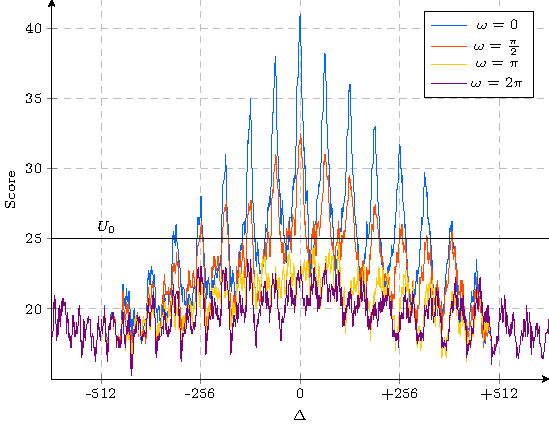
\includegraphics[width=\linewidth, height=.75\textheight, keepaspectratio=true]{figures/pgfplots/score_function_stdl.pdf}
    \end{column}
  \end{columns}
  \note{
    \begin{enumerate}
      \item Rappel, en vrai les systèmes sont imparfaits \dots
      \item Doppler, horloge
      \item freq => rotation. Plus simple de considérer symbole.
      \item $+$ on est aveugle  !
    \end{enumerate}
  }
\end{frame}

\begin{frame}{\subsecname : {La grille temps fréquences}}
  \begin{columns}
    \begin{column}{.6\linewidth}
      \begin{ctrlitemize}{6pt}
        \item Ouverture d'une fenêtre de détection, de taille $\textcolor{Red}{\mpd} \times \textcolor{Blue}{\mpo}$.
        \item Calcul de $\textcolor{Red}{\mpd}$ valeurs de scores tous les $q$ chips : $\searrow$ de la complexité, $\searrow$ de performances de détection.
        \item Calcul de $\textcolor{Blue}{\mpo}$ valeurs de scores sur un intervalle arbitraire (ex: $2\pi$) : $\nearrow$ des performances de détection, $\nearrow$ de la complexité.
      \end{ctrlitemize}
    \end{column}
    \begin{column}{.4\linewidth}
      \centering
      \includegraphics[width=\linewidth, height=.85\textheight, keepaspectratio=true]{figures/pgfplots/score_grid.pdf}
    \end{column}
  \end{columns}
  \note{
    \begin{enumerate}
      \item Solution : La grille (you know what to say)
      \item PS wink wink : dans les travaux théorique, pas de \pd{} ni \po{} mais vu \Delta / \omega, c'est moi qui ai introduit pour imple' purpose
      \item Slide suivante, c'est le résumé en modèle fonctionnel, BG
    \end{enumerate}
  }
\end{frame}

\begin{frame}{\subsecname : {Modèle fonctionnel}}
  \begin{center}
    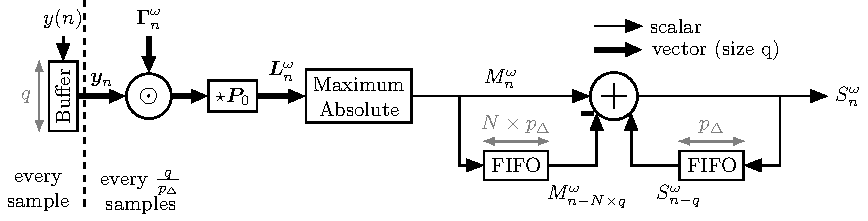
\includegraphics[
      width=.75\linewidth,
      height=.35\textheight,
      keepaspectratio=true
    ]{figures/tikzpicture/score_proc_unit_legacy_stdl.pdf}

    \vspace{1em}

    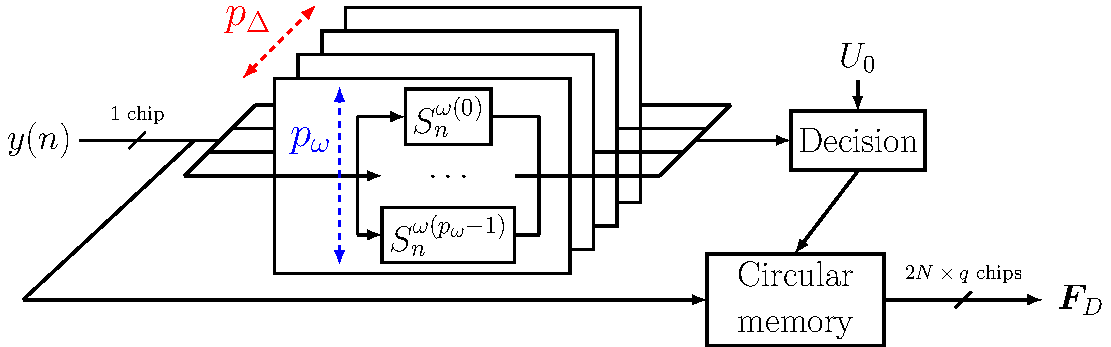
\includegraphics[
      width=.9\linewidth,
      height=.4\textheight,
      keepaspectratio=true
    ]{figures/tikzpicture/funct_view_detection_stdl.pdf}
  \end{center}
  \note{
    \begin{enumerate}
      \item $\mpd{} \times \mpo{}$ scores $\heartsuit$
    \end{enumerate}
  }
\end{frame}

\begin{frame}{\subsecname : {Effets des paramètres $p_\Delta$ et $p_\omega$}}{Données réelles avec $q = 64$ et $N = 60$}
  \begin{overlayarea}{\linewidth}{.15\textheight} \vspace {-1.2cm}
    \hfill 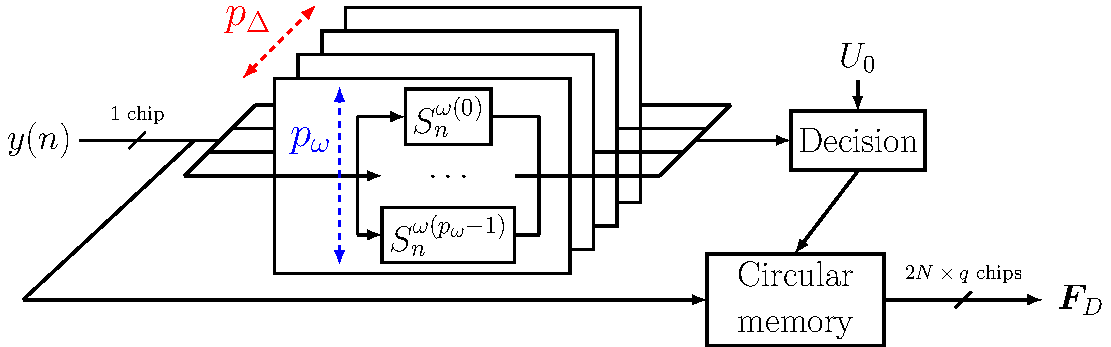
\includegraphics[width=6.5cm, height=.75\textheight, keepaspectratio=true]{figures/tikzpicture/funct_view_detection_stdl.pdf}
  \end{overlayarea}
  \begin{columns}
    \begin{column}{.65\linewidth}
      \begin{overlayarea}{\linewidth}{.75\textheight} \vspace {-.5cm}
        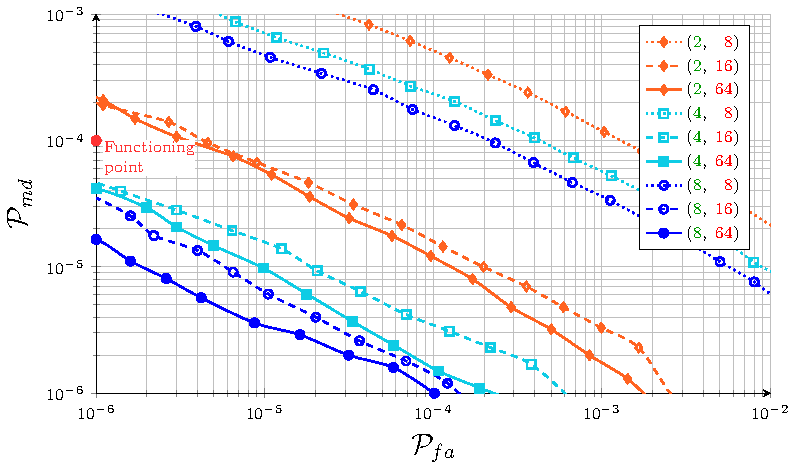
\includegraphics[width=\linewidth]{pgfplots/roc_curves_stdl.pdf}
      \end{overlayarea}
    \end{column}
    \begin{column}{.35\linewidth} \vspace {-.5cm}
      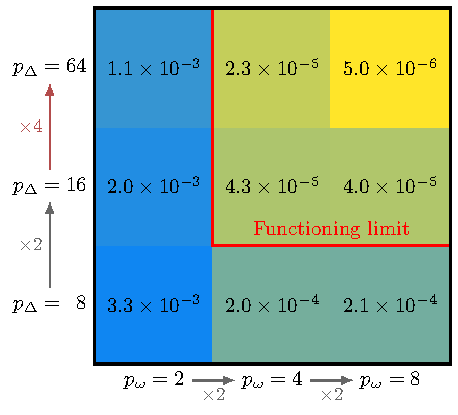
\includegraphics[width=\linewidth]{pgfplots/popw_maps_m10dB_60x64_stdl.pdf}
    \end{column}
  \end{columns}
  \note{
    ``Pour finir cet état des lieux''
    \begin{enumerate}
      \item $\mpd{}$ et $\mpo{}$ -> impact sur perfo. de dét. et complexité
      \item Ici c'est ROC et déroule
      \begin{itemize}
        \item \acrfull{pfa}
        \item \acrfull{pmd}
        \item best détecteur : PFA = PMD = 0 <=> Il détecte \textbf{que} les trames, et \textbf{toutes} les trames. 
      \end{itemize}
      \item Mais \pd{} et \po{}, c'est pas yolo ! (les couleurs TMTC)
    \end{enumerate}
  }
\end{frame}

% \subsection{Synchronisation et décodage}

% \begin{frame}{\subsecname}
%   \begin{center}
%     \textcolor{RoyalBlue}{TODO --- En fonction du temps, détails ou pas}
%   \end{center}
% \end{frame}

% \subsection{Décodage}

\begin{frame}{\subsecname}
  \begin{center}
    
    \includegraphics[width = .9\linewidth]{figures/tikzpicture/chain_matlab.pdf}
  \end{center}
  \begin{columns}
    \begin{column}{.8\linewidth}
      \begin{itemize}
        \item La chaine existe \dots en \textsc{Matlab} :
        \begin{itemize}
          \item Suffisante pour les simulations ;
          \item Montre des limites pour les simulations intensives ;
          \item Impossible de l'utiliser en conditions réelles ou en temps réel.
        \end{itemize}
      \end{itemize}
    \end{column}
  \end{columns}
  \note{
    Le temps réel, j'le bouffe au p'tit déj.
  }
\end{frame}

\end{document}
